\documentclass{beamer} 
\usepackage[latin1]{inputenc}
\usepackage[english]{babel}
\usetheme{CambridgeUS}

% page formating
\setlength{\parindent}{0pt}

% fonts
\usefonttheme{professionalfonts}
\usefonttheme[onlymath]{serif}
\usepackage{amsmath, bm}

% ??
%\usepackage{times}

% code and psendocode
\usepackage{verbatim}
\usepackage{minted}
\usemintedstyle{trac}
\usepackage{algorithm, algorithmic}

% colors
\usepackage{xcolor}
\definecolor{LightGray}{gray}{0.95}
\definecolor{DarkGray}{gray}{0}

% new commands
\newcommand{\real}{\mathbb{R}}
\newcommand{\bernoulli}{\mathrm{Bernoulli}}
\newcommand{\relu}{\mathrm{relu}}
\newcommand{\sig}{\mathrm{sigmoid}}
\newcommand{\kldiv}{\mathcal{D}_{KL}}
\newcommand{\E}{\mathrm{E}}
\newcommand{\encoder}{\mathrm{encoder}}
\newcommand{\code}[1]{{\small\colorbox{LightGray}{\texttt{#1}}}}

% title page
\title{Machine Learning Workshop 2}
\subtitle{Variational Autoencoder}
\author{Jonathan~Guymont}
\date{National Bank of Canada, 2018}

\AtBeginSubsection[]
{
    \begin{frame}<beamer>{Outline}
        \tableofcontents[currentsubsection]
    \end{frame}
}

\begin{document}

\begin{frame}
	\titlepage 
\end{frame}

\begin{frame}{Outline}
	\tableofcontents
\end{frame}

\section{Autoencoders}

\subsection{An example to keep in mind}

\begin{frame}[fragile]{An example to keep in mind}
\begin{figure}
	\centering
	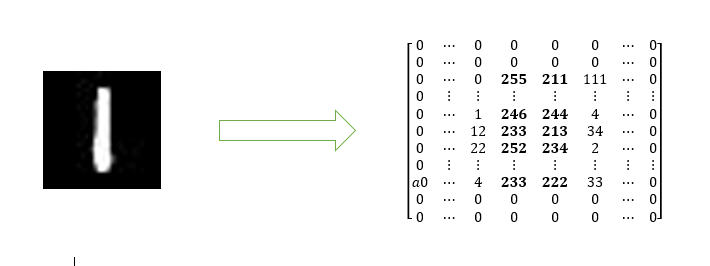
\includegraphics[scale=0.3]{image_to_array}
	\caption{Conversion of a greyscale image to an matrix}
\end{figure}
Note: In the workshop, we will mostly work with linear layer, so we also need to flatten the image.
\begin{minted}[bgcolor=LightGray, fontsize=\footnotesize]{python}
from PIL import Image
def image_to_array(image_path):
    with Image.open(image_path) as img:
        image = img.convert()
        array_image = np.asarray(image, np.float)
    return array_image
\end{minted}
\end{frame}

\subsection{Autoencoders}

\begin{frame}{Autoencoders}
Autoencoers are neural network that are trained to learn how to map their input to their input. Internally, it has an hidden layer $\bm{h}$ that contains a lossy summary of the relevant feature for the task.
\end{frame}
  
\begin{frame}{Autoencoders}
An autoencoder can be seen has a two parts network
\begin{itemize}
	\item Encoder function: $\bm{z}=f_\phi(\bm{x})$
	\item Decoder function: $\tilde{\bm{x}} = g_\theta(\bm{z})$
	\item $\phi$ and $\theta$ are set of learned parameters
\end{itemize}
\end{frame}

\begin{frame}{Autoencoders}
	The simplest autoencoder is a one layer MLP:
	\Large
	\begin{equation}
	\begin{split}
		\mathbf{z} =& \relu\left(\mathbf{W}_{xz}\mathbf{x}+\mathbf{b}_{xz}\right)~~[\text{encoder}]\\
		\tilde{\mathbf{x}} =& \sig\left(\mathbf{W}_{zx}\mathbf{z}+\mathbf{b}_{zx}\right)~~[\text{decoder}]
	\end{split}
	\end{equation}
\end{frame}

\begin{frame}[fragile]{Pytorch simple autoencoder}
\begin{minted}[bgcolor=LightGray, fontsize=\footnotesize]{python}
class Autoencoder:
	def __init__(self, **kargs):
	    """constructor"""
	    pass
	
	def encoder(self, x):
	    pass
	
	def decoder(self, z)
	    pass
	    
	def forward(self, x):
	    pass
\end{minted}
\end{frame}

\begin{frame}[fragile]{Parameter initialization}
\begin{equation}
\begin{split}
\mathbf{z} =& \relu\left(\mathbf{W}_{xz}\mathbf{x}+\mathbf{b}_{xz}\right)\\
\tilde{\mathbf{x}} =& \sig\left(\mathbf{W}_{zx}\mathbf{z}+\mathbf{b}_{zx}\right) 
\end{split}
\end{equation}
\begin{minted}[bgcolor=LightGray, fontsize=\footnotesize]{python}
class Autoencoder:
    def __init__(self, x_dim, z_dim):
        # encoder parameters \phi
        self.Wxz = xavier_init(size=[x_dim, z_dim])
        self.bxz = Variable(torch.zeros(z_dim), requires_grad=True)
        # decoder parameters \theta
        self.Wzx = xavier_init(size=[z_dim, x_dim])
        self.bzx = Variable(torch.zeros(x_dim), requires_grad=True)
\end{minted}
\end{frame}

\begin{frame}[fragile]{Encoder $f_\phi(x)$}
\begin{align}
	\mathbf{z} =& \relu\left(\mathbf{W}_{xz}\mathbf{x}+\mathbf{b}_{xz}\right)\\
	\bm{\phi}=&\{\mathbf{W}_{xz}, \mathbf{b}_{xz}\} 
\end{align}
\begin{minted}[bgcolor=LightGray, fontsize=\footnotesize]{python}
class Autoencoder:
        ...
    def encoder(self, x):
        z = F.relu(self.Wxz @ z + self.bxz.repeat(x.size(0), 1))
        return z
\end{minted}
\end{frame}

\begin{frame}[fragile]{Decoder $g_\theta(x)$}
\begin{align}
	\mathbf{z} 
	=& \sigma\left(\mathbf{W}_{zx}\mathbf{z}+\mathbf{b}_{zx}\right)\\
\bm{\theta}=&\{\mathbf{W}_{zx}, \mathbf{b}_{zx}\} 
\end{align}
\begin{minted}[bgcolor=LightGray, fontsize=\footnotesize]{python}
class Autoencoder:
        ...
    def decoder(self, z):
        x_recon = F.sigmoid(z @ self.Wzx + self.bzx.repeat(z.size(0), 1))
        return x_recon
\end{minted}
\end{frame}

\begin{frame}[fragile]{Forward propagation}
\begin{equation}
\begin{split}
\mathbf{z} =& \relu\left(\mathbf{W}_{xz}\mathbf{x}+\mathbf{b}_{xz}\right)\\
\tilde{\mathbf{x}} =& \sig\left(\mathbf{W}_{zx}\mathbf{z}+\mathbf{b}_{zx}\right) 
\end{split}
\end{equation}
\begin{minted}[bgcolor=LightGray, fontsize=\footnotesize]{python}
class Autoencoder:
        ...
    def forward(self, x):
        z = self.encoder(x)
        x_recon = self.decoder(z)
        return x_recon
\end{minted}
\end{frame}

\begin{frame}[fragile]{Pytorch simple autoencoder}
\begin{minted}[bgcolor=LightGray, fontsize=\tiny]{python}
class Autoencoder:
    def __init__(self, x_dim, z_dim):
        # encoder parameters
        Wxz = xavier_init(size=[x_dim, z_dim])
        bxz = Variable(torch.zeros(z_dim), requires_grad=True)
        # decoder parameters
        Wzx = xavier_init(size=[h_dim, x_dim])
        bzx = Variable(torch.zeros(X_dim), requires_grad=True)
    
    def encoder(self, x):
        z = F.relu(x @ self.Wxh + self.bxh.repeat(x.size(0), 1))
        return z
    
    def decoder(self, z):
        x_recon = F.sigmoid(z @ self.Wzx + self.bzx.repeat(z.size(0), 1))
        return x_recon
    
    def forward(self, x):
        z = self.encoder(x)
        x_recon = self.decoder(z)
        return x_recon
\end{minted}
\end{frame}

\begin{frame}{Autoencoder - Loss Function}
If you treat the problem like a \textit{regression}\footnote{If you do regression, you don't have to apply sigmoid in the decoder.}, use the mean square error between the input and the reconstruction
\begin{equation}
\mathcal{L} = \sum_{i=1}^d (x_i-\tilde{x}_i)^2
\end{equation}
\end{frame}

\begin{frame}{Training Autoencoders}
\begin{algorithm}[H]
	\begin{algorithmic}
		\REQUIRE Learning rate $\eta$
		\REQUIRE Initial parameter $\bm{\omega}_0$
		\REQUIRE Number of epochs $T$
		\FOR{$i=1$ to $T$}
		\STATE $X =X^{train}$.copy() and $Y =Y^{train}$.copy()
		\WHILE{$X$ is not empty}
		\STATE Sample $\{x^{(1)},...,x^{(m)}\}$ from $X$ and $\{y^{(1)},...,y^{(m)}\}$ from $Y$
		\STATE Remove samples from $X$ and $Y$
		\STATE Compute gradient $\bm{g}_t=\frac{1}{m}\nabla_{\bm{\omega}}\sum_i \mathcal{L}(\tilde{x}^{(i)}, x^{(i)})$  
		\STATE Apply update: $\mathbf{\omega}_t=\bm{\omega}_{t-1}-\eta\cdot \bm{g}_t$
		\ENDWHILE
		\ENDFOR
	\end{algorithmic}
	\caption{Pseudocode for Stochastic Gradient Training}
	\label{alg:sgd}
\end{algorithm}
\end{frame}

\begin{frame}[fragile]{Pytorch Stochastic Gradient}
\begin{minted}[bgcolor=LightGray, fontsize=\tiny]{python}
def train(self, trainloader, num_epochs, learning_rate):

    for epoch in range(num_epochs):
        for inputs, targets in trainloader:
            batch_size = inputs.size(0)
            x_tilde = self.forward(x)

            loss = F.mse_loss(x, x_tilde)

            # Use autograd to compute the derivative of the loss w.r.t 
            # all Tensors with requires_grad=True. After calling `loss.backward()`, 
            # conv_weight.grad, dense_weight.grad, and dense_bias.grad 
            # will be Tensors equal to the gradient of the loss with respect 
            # to the filters of the cnn layer, the weight of the fully connected layer, and 
            # the bias of the fully connected layer respectively.
            loss.backward()
            
            # Apply gradient descent to all the leaned parameters
            # The derivative of the loss is giving us the direction
            # where the funtion increase. Thus we go in the 
            # opposite direction. Using torch.no_grad() tells pytorch
            # to not include thes operation in the computational graph.
            # Instead, gradient descent is goning to be applied `inplace`.
            with torch.no_grad():
                self.W_xz -= learning_rate * self.W_xz.grad
                self.b_xz -= learning_rate * self.b_xz.grad
                self.W_zx -= learning_rate * self.W_zx.grad
                self.b_zx -= learning_rate * self.b_zx.grad
\end{minted}
\end{frame}

\begin{frame}{Autoencoders}

To summarize
\begin{itemize}
	\item A neural network encode $x$ in a hidden state $z$ of smaller dimension
	\item Another neural network decode $z$ to reconstruct $x$
	\item A sound loss function could be the mean square error between the input and its reconstruction.
	\item Both network can be train at the same time with gradient method.
\end{itemize}
\end{frame}

\section{Variational autoencoder}

\subsection{Generative Model}

\begin{frame}{Generative Models}
Represent the probability distribution of either $P(X,Y)$ or $P(X)$. In the case of \textit{density estimation}, we are looking for a representation of

\huge
\[
	x \sim P_\theta(X)
\]
\normalsize
For example, $x\sim \mathcal{N}(x;\bm{\mu}_{\text{mle}}, \bm{\sigma}_{\text{mle}})$ \\

Problem: Most parametric distribution make strong (and often wrong) assumption about the distribution.
\end{frame}

\subsection{Latent variable models}

\begin{frame}{Latent variable models}
	We can model the distribution of $x$ as a function of a latent variable $z$
	\[
	p(x) = \int p_\theta (x|z) p(z) dz
	\]
	where the distribution of $z$ is chosen. A typical choice for $z$ is 
	\[
		z\sim \mathcal{N}(z;\bm{0}, \bm{I})
	\]
	Then we can train a model to learn a good representation of $p_\theta (x|z)$ with stochastic gradient.
\end{frame}

\begin{frame}{Latent variable models}
	\[
		p(x) = \int p_\theta (x|z) p(z) dz
	\]
	Once we have a good representation of $p_\theta (x|z)$, we can sample from $p(x)$ by first sampling
	\[
		z'\sim p(z)
	\]
	and then sampling\\
	\[
		x'\sim p(x|z')
	\]
\end{frame}

\begin{frame}{Latent variable models}
	Problem 1: To learn $p_\theta(x|z)$ using stochastic gradient, we need to know a good mapping 
	\[
		f: \mathcal{Z}\times \Theta \mapsto \mathcal{X}
	\]
	In other word when we sample $x\sim p(x|z')$ we need to know which $x$ is likely to be generated by this particular $z'$ in order to train the model.
\end{frame}

\begin{frame}{Latent variable models}
	Solution: the prior of the latent space can be written has
	\[
	p(z) = \int p(z|x) p(x) dx
	\]
	During training, We can sample $z$ by sampling \\
	\[
	x'\sim p(x)
	\]
	and then 
	\[z\sim p(z|x')\]
	
	 The training set comes from $p(x)$ so we can sample from it. This will reduce the space of the latent variable a lot and allow the model to learn efficiently.
\end{frame}

\begin{frame}{Latent variable models}
	Problem 2: $p(z|x)$ is intractable. \\
	
	Solution: use an approximation $q_\phi(z|x)$\\
	
	To summarize
	\begin{itemize}
		\item Sample $x \sim D_n$
		\item Sample $z \sim q_\phi(z|x)$
		\item Sample $\tilde{x} \sim p_\theta(x|z)$
	\end{itemize}
	The parameter to learn are $\phi$ and $\theta$ and they should be learn such that the marginal likelihood $p(x)$ is maximized.
\end{frame}

\begin{frame}{Latent variable models}
	Before looking at how we can train this model efficiently, let's take a closer look at how it works concretely.
\end{frame}

\begin{frame}[fragile]{Probabilistic Encoder $q_\phi(z|x)$}
	Example: Gaussian MLP as encoder
	\begin{itemize}
		\item $\bm{\mu}_z,~\log\bm{\sigma}_z^2=f(\mathbf{x};\bm{\phi})$
		\begin{itemize}
			\item $\mathbf{h} = \relu\left(x W_{xh}+b_{xh}\right)$
			\item $\mu = h W^{(1)}_{hz}+b^{(1)}_{hz}$
			\item $\log \sigma^2 = h W^{(2)}_{hz}+b^{(2)}_{hz}$
		\end{itemize}
		\item $q_\phi(z|x)=\mathcal{N}(\mathbf{z};\bm{\mu}_z, \bm{\sigma}_z^2)$
		\item $\phi = \{W^{(1)}_{hz}, b^{(1)}_{hz}, W^{(2)}_{hz}, b^{(2)}_{hz}, W_{xh}, b_{xh}\}$
	\end{itemize}
\begin{minted}[bgcolor=LightGray, fontsize=\footnotesize]{python}
class VAE:
    ...
    def encoder(self, x):
        # Encoder network. Return the parameter of q(z|x)
        h = relu(x @ self.Wxh + self.bxh.repeat(x.size(0), 1))  
        mu = h @ self.Whz_mu + self.bhz_mu.repeat(x.size(0), 1)      
        log_var = h @ self.Whz_var + self.bhz_var.repeat(x.size(0), 1)
        reture mu, log_var
\end{minted}
\end{frame}

\begin{frame}[fragile]{Sampling $z\sim q_\phi(z|x)$}
Example: Sampling $z$ from $q_\phi(z|x)$
\begin{itemize}
	\item $\mathbf{z}\sim \mathcal{N}(\bm{\mu}_z, \bm{\sigma}_z)$
	\begin{itemize}
		\item $\bm{\mu}_z,~\log\bm{\sigma}^2_z=f(\mathbf{x};\bm{\phi})$
		\item $\bm{\epsilon} \sim \mathcal{N}(\mathbf{0}, \mathbf{I})$
		\item $\mathbf{z} = \bm{\mu}_z + \bm{\sigma}_z \odot \bm{\epsilon} $
	\end{itemize}
\end{itemize}
\begin{minted}[bgcolor=LightGray, fontsize=\footnotesize]{python}
class VAE:
    ...
    def _sample_z(self, mu, log_var):
        epsilon = Variable(torch.randn(mu.size()).to(self._device)
        sigma = torch.exp(log_var / 2)
        return mu + sigma * epsilon
\end{minted}
\end{frame}

\begin{frame}[fragile]{Probabilistic Decoder $p_\theta(x|z)$}
	Example: Gaussian MLP as decoder
	\begin{itemize}
		\item $\bm{\mu}_x,~\log\bm{\sigma}_x^2=g(\mathbf{x};\bm{\theta})$
		\begin{itemize}
			\item $\mathbf{h} = \relu\left(\mathbf{W}_{zh}\mathbf{x}+\mathbf{b}_{zh}\right)$
			\item $\bm{\mu}_x = W^{(1)}_{hz}\mathbf{h}+\mathbf{b}^{(1)}_{hz}$
			\item $\log \bm{\sigma}_x^2 = W^{(2)}_{hz}\mathbf{h}+\mathbf{b}^{(2)}_{hz}$
		\end{itemize}
		\item $p_{\bm{\theta}}(x|z)=\mathcal{N}(x;\bm{\mu}_x, \log\bm{\sigma}_x^2)$
		\item $\bm{\theta} = \{W_{zh}, b_{zh}, W_{zx}, b_{zx}\}$
	\end{itemize}
\begin{minted}[bgcolor=LightGray, fontsize=\footnotesize]{python}
class VAE:
    ...
    def decoder(self, z):
        # Decoder network. Reconstruct the input from 
        # the latent variable z
        h = relu(z @ self.Whx + self.bhx.repeat(x.size(0), 1))  
        gamma = h @ self.Whx_mu + self.bhx.repeat(x.size(0), 1)      
        reture gamma
\end{minted}
\end{frame}

\begin{frame}{Latent variable models}
	To summarize
	\begin{itemize}
		\item Sample $x \sim D_n$
		\item Sample $z \sim q_\phi(z|x)$
		\item Sample $\tilde{x} \sim p_\theta(x|z)$
	\end{itemize}
	The parameter to learn are $\phi$ and $\theta$ and they should be learn such that the marginal likelihood $p(x)$ is maximized.
\end{frame}

\subsection{Variational Lower Bound}

\begin{frame}{Training VAE}
	We need $p_\theta(x|z)$ to be such that the marginal likelihood $p(x)$ is maximized. \\
	
	In other word the lost function should be
	\[
		-\log p(x^{(1)},...,x^{(N)}) = -\sum_{i=1}^N \log p(x^{(i)})
	\]
\end{frame}

\begin{frame}{Kullback-Leibler divergence}
	\begin{equation}
		\kldiv[q(x)||p(x)] 
		= \E_{x\sim q(x)}[ \log q(x) - \log p(x)]
	\end{equation}

	\bigskip

	Gibbs' inequality:
	\begin{equation}
		\kldiv[q(x)||p(x)] \geq 0
	\end{equation}
\end{frame}

\begin{frame}{Training VAE}
	Now let's compute de Kullback-Leibler divergence $\kldiv$ between $p(z|x)$ and $q(z|x)$
	%\scriptsize
	\begin{equation*}
	\begin{split}
		\kldiv[q(z|&x)||p(z|x)]\\ 
		=& \E_{z\sim q(z|x)}[ \log q(z|x) - \log p(z|x)]\\
		=& \E_{z\sim q(z|x)}[ \log q(z|x) - \log p(x|z) - \log p(z) + \log p(x)]\\
		=& \log p(x) + \E_{z\sim q(z|x)}[ \log q(z|x)  - \log p(z)] - \E_{z\sim q(z|x)}\log p(x|z)\\
		=& \log p(x) - \kldiv[q(z|x)||p(z|x)] - \E_{z\sim q(z|x)}\log p(x|z)\\
	\end{split}
	\end{equation*}
\end{frame}

\begin{frame}{Training VAE}
	\small
	\begin{equation}
	\begin{split}
		\log p(x) = \E_{z\sim q(z|x)}\log p(x|z)- \kldiv[q(z|x)||p(z)] + \kldiv[q(z|x)||\log p(z|x)]\\
	\end{split}
	\end{equation}
	\normalsize
	Because of Gibbs' inequality we have
	\[
		\log p(x)  \geq \E_{z\sim q(z|x)}\log p(x|z)- \kldiv[q(z|x)||p(z)]
	\]
	Hence, our loss function is
	\[
		\mathcal{L} = \E_{z\sim q(z|x)}\log p(x|z)- \kldiv[q(z|x)||p(z)]
	\]
\end{frame}

\begin{frame}{Solution of $\kldiv[q(z|x)||p(z)]$}
	\begin{equation*}
	\begin{split}
		\kldiv[q_\phi(z|x)||p(z)] 
		=& \int q_\phi(z|x)(\log q_\phi(z|x)-\log p(z))dx\\
		=& \int q_\phi(z|x)\log q_\phi(z|x)dx-\int q_\phi(z|x)\log p(z))dx
	\end{split}
	\end{equation*}
\end{frame}

\begin{frame}{Training VAE}
	Suppose $z\in \real^J$ is normal 
	\begin{equation}
	\begin{split}
		\int q(z|x)\log q(z|x)dz =& \int \mathcal{N}(z;\mu, \sigma)\log \mathcal{N}(z;\mu, \sigma)\\
		=& -\frac{J}{2} \log 2\pi - \frac{1}{2}\sum_{j=1}^J (1+\log \sigma_j^2)
		\end{split}
		\label{eq:klgauss1}
	\end{equation}
	\begin{equation}
	\begin{split}
		\int q(z|x)\log p(z)dz =& \int \mathcal{N}(z;\mu, \sigma)\log \mathcal{N}(z;0, I)\\
		=& -\frac{J}{2} \log 2\pi - \frac{1}{2}\sum_{j=1}^J (\mu_j^2+\sigma_j^2)
		\end{split}
		\label{eq:klgauss2}
	\end{equation}
\end{frame}

\begin{frame}[fragile]{Training VAE}
	\begin{equation}
	\begin{split}
		\kldiv[q(z|x)||p(z)] =& (\ref{eq:klgauss1})-(\ref{eq:klgauss2})\\
		=& \frac{1}{2}\sum_{j=1}^J \mu_j^2 + \sigma_j^2 - 1 - \log \sigma_j^2
	\end{split}
	\end{equation}
\begin{minted}[bgcolor=LightGray, fontsize=\footnotesize]{python}
def kl_divergence(mu, log_sigma):
    sigma = torch.exp(log_sigma)
    return .5 * torch.sum(mu**2 + sigma**2 - 1 - 2*log_sigma, axis=1)
\end{minted}
\end{frame}

\begin{frame}[fragile]{VAE Loss Function}
\begin{equation}
\begin{split}
		\mathcal{L} 
		=& -\E_{z\sim q(z|x)}\log p(x|z) + \kldiv[q(z|x)||p(z)]\\
		=& -\log \mathcal{N}(x;\bm{\mu}_x, \bm{\sigma}_x) + \frac{1}{2}\sum_{j=1}^J \mu_j^2 + \sigma_j^2 - 1 - \log \sigma_j^2
\end{split}
\end{equation}
\end{frame}

\section{Experiment}

\subsection{Unsupervised Spam Detection}

\begin{frame}{Unsupervised Spam Detection}
\begin{itemize}
	\item SMS Spam Collecion Data Set\footnote{https://archive.ics.uci.edu/ml/datasets/sms+spam+collection}\begin{itemize}
		\item Number of instances: 5574
		\item Number of spams: 747 ($\sim 13 \%$)
	\end{itemize} 
	\item Spam detection
	\begin{itemize}
		\item Estimate the distribution of all the text messages
		\item Evaluate the density of each text message
		\item Text message with low density are classified as spam
	\end{itemize}
\end{itemize}
\end{frame}

\begin{frame}{Data}
\begin{itemize}
	\item Examples of \textbf{non spams}
	\begin{itemize}
		\item \textit{What you doing?how are you?}
		\item \textit{Ok lar... Joking wif u oni...} 
		\item \textit{Cos i was out shopping wif darren jus now n i called him 2 ask wat present he wan lor. Then he started guessing who i was wif n he finally guessed darren lor.}
	\end{itemize} 
	\item Examples of \textbf{spams}
	\begin{itemize}
		\item  \textit{FreeMsg: Txt: CALL to No: 86888 \& claim your reward of 3 hours talk time to use from your phone now! ubscribe6GBP/ mnth inc 3hrs 16 stop?txtStop}
		\item  \textit{Sunshine Quiz! Win a super Sony DVD recorder if you canname the capital of Australia? Text MQUIZ to 82277. B}
		\item \textit{URGENT! Your Mobile No 07808726822 was awarded a L2,000 Bonus Caller Prize on 02/09/03! This is our 2nd attempt to contact YOU! Call 0871-872-9758 BOX95QUm}
	\end{itemize}
\end{itemize}
\end{frame}

\begin{frame}{Performance Metric}
\begin{equation}
	\begin{split}
		\mathrm{F_1-Score} =&
		\left(\frac{\mathrm{recall}^{-1} + \mathrm{precision}^{-1}}{2}\right)^{-1}\\
		=&
		2\cdot \frac{\mathrm{precision}\cdot \mathrm{recall}}{\mathrm{precision}+\mathrm{recall}}
	\end{split}
	\end{equation}
	where 
	\begin{equation*}
	\mathrm{precision} = \frac{|\{\mathrm{spams~detected}\}|}{|\{\mathrm{spams~classified}\}|}
	~~~~~
	\mathrm{recall} = \frac{|\{\mathrm{spams~detected}\}|}{|\{\mathrm{spams}\}|}
	\end{equation*}
	Motivation: Both precision and recall metric are important. Take the harmonic mean between them.
\end{frame}

%\begin{frame}{Anomaly detection and autoencoder}
%	Some anomaly detection methods:
%	\begin{itemize}
%		\item Statistical: A data point is defined as an anomaly if the density of it being generated from the model is below a threshold
%		\item Proximity based: A data point is defined as an anomaly if it is \textit{islolated} (e.g. far from clusters centroid)
%		\item Deviation based: Use reconstruction error to detect anomaly (e.g. $k$-most significant principle component (PCA) and autoencoders based methods)
%	\end{itemize}
%\end{frame}

\subsection{Preprocessing}

\begin{frame}{Preprocessing}
	\begin{itemize}
		\item Some terminology
		\begin{itemize}
			\item Vocabulary: Set of all the word types in the training set $\{w_1,...,w_{|\text{Vocabulary}|}\}$.
			\item Training corpus: Set of all text messages in the training set $\{x^{(1)},...,x^{(n)}\}$.
			\item Bag of words: Vector representation of a sentence.
		\end{itemize}
	\end{itemize}
\end{frame}

\begin{frame}[fragile]{Bag of words}
	\begin{itemize}
		\item $x^{(i)}=\textit{What you doing?how are you?}$ (original sentence)
		\item $x^{(i)}=\textit{what you do how be you}$ (after preprocessing)
		\item $x^{(i)}=[0\cdots0~1~0\cdots~0~2~0\cdots0]$ (vector representation)
	\end{itemize}
\begin{minted}[bgcolor=LightGray, fontsize=\footnotesize]{python}
x = 'What you doing?how are you?'

x = preprocess(x)
print(x)
>>> 'what you do how be you'

x = vectorize(x)
print(x)
>>> [0 0 0 ... 0 0 0]
\end{minted}
\end{frame}

\begin{frame}[fragile]{Bag of words}
\begin{itemize}
	\item Bag of words
	\begin{itemize}
		\item All examples in the corpus have the same length. 
		\item The value of a position in the vector is equal to the frequency of this word it the example.
		\item $x^{(i)}=[0\cdots0~1~0\cdots~0~2~0\cdots0]$
	\end{itemize}
	\item Binary bag of words
	\begin{itemize}
		\item All examples in the corpus have the same length. 
		\item Each element in the vector is either 0 or 1.
		\item $x^{(i)}=[0\cdots0~1~0\cdots~0~1~0\cdots0]$
	\end{itemize}
\end{itemize}
\end{frame}

\subsection{Binary Cross Entropy}

\begin{frame}{Binary Cross Entropy}
	Recall that the density of a Bernoulli distribution is given by 
	\begin{equation}
	\bernoulli(x;\gamma) = \gamma^x(1-\gamma)^{1-x}
	\end{equation}
	where $\gamma\equiv p(x=1)$.
\end{frame}

\begin{frame}{Binary Cross Entropy}
	Thus the log-likelihood of a Bernoulli distribution is
	\begin{equation}
	\log p(x) = x\log\gamma + (1-x)\log(1-\gamma)
	\end{equation}
\end{frame}

\begin{frame}[fragile]{Binary Cross Entropy}
	If your have binary features, i.e. $x_i\in \{0,1\}$ for $i=1,...,d$, then the output of the decoder can be interpreted has the parameter of a Bernoulli. Thus the likelihood of the input $x$ can be compute has 
	\begin{equation}
	p(x|z)=\prod_{i=1}^dp(x_i|z) = \prod_{i=1}^d\gamma_i^{x_i}(1-\gamma_i)^{1-x_i}
	\end{equation}
	Note that this works only if $\gamma_i\in (0, 1)$. To ensure it, apply sigmoid element wise on the output of the decoder.
\end{frame}

\begin{frame}[fragile]{Binary Cross Entropy}
And the log-likelihood is given by
	\begin{equation*}
	\log p(x|z) = -\sum_{i=1}^d x_i\log \gamma_i + (1-x_i)\log(1-\gamma_i) 
	\end{equation*}
\begin{minted}[bgcolor=LightGray, fontsize=\footnotesize]{python}
# in pytorch
functional.binary_cross_entropy(param, x)
\end{minted}
\end{frame}

\subsection{Bernoulli MLP as Decoder}

\begin{frame}[fragile]{Probabilistic Decoder $p_\theta(x|z)$}
Bernoulli MLP as decoder
\begin{itemize}
	\item $\bm{\gamma}=g(z;\bm{\theta})$
	\begin{itemize}
		\item $h = \relu\left(W_{zh}x+b_{zh}\right)$
		\item $\gamma = \sigma\left(W_{hx}h+b_{hx}\right)$
	\end{itemize}
	\item $p_\theta(x|z)=\bernoulli(x;\bm{\gamma})$
	\item $\bm{\theta} = \{W_{zh}, b_{zh}, W_{zx}, b_{zx}\}$
\end{itemize}
\begin{minted}[bgcolor=LightGray, fontsize=\footnotesize]{python}
class VAE:
    ...
    def decoder(self, z):
        h = relu(self.W_zh @ z + self.b_zh.repeat(x.size(0), 1))  
        gamma = self.W_hx @ h + self.b_hx.repeat(x.size(0), 1)      
        reture gamma
\end{minted}
\end{frame}

\subsection{Spam Detector}

\begin{frame}{Anomaly detection}  
\begin{algorithm}[H]
	\begin{algorithmic}
		\REQUIRE Learning rate $\epsilon_k$
		\REQUIRE Initial parameter $\bm{w}_0$
		\REQUIRE Number of epochs $T$
		\FOR{$i=1$ to $T$}
		\STATE Compute gradient $\bm{g}_t=\frac{1}{m}\nabla_w\sum_i L(h_{w_{t-1}}(\bm{x}^{(i)}), \bm{y}^{(i)})$ 
		\STATE Apply update: $\bm{w}_t=\bm{w}_{t-1}-\epsilon \bm{g}_t$
		\ENDFOR
	\end{algorithmic}
	\caption{Pseudocode for Batch Gradient Descent}
	\label{alg:se}
\end{algorithm}
\end{frame}




\end{document}